\chapter{Evaluation of Neural Network Models} \label{chap:eval_NN}
This chapter examines the applications of non-Bayesian and Bayesian neural networks using two datasets. First a dataset on housing prices in Boston for regression and secondly a dataset on credit card client defaults for classification. We will evaluate the models by comparing and examining their accuracy as well as computational runtime.
\\
\\
All models are implemented in the programming language Python and the code can be found in the appendix. The specification on the computer that has performed the computation of the models are shown in appendix \ref{app:specs} along with the packages used and their versions.
\\
\\
In section \ref{sec:Boston_housing} we examine the median prices on houses in specific areas of Boston based on a number of features shown in table \ref{tab:Boston_Housing}. We aim to predict unknown median prices based on these features using regression. Section \ref{sec:credit_default} examines defaulting payments on credit card clients in Taiwan. Our objective is in this case to predict the probability of defaults and describe how these can be used for classifying whether a client will default or not.

\section{Predicting House Prices in Boston} \label{sec:Boston_housing}
The Boston housing data was originally introduced by \cite{HARRISON197881}, who investigated the effect of air pollution on house prices.
The dataset contains information collected by the U.S Census Service concerning housing in the area of Boston Massachusetts. The sample contains 506 examples, where each example represents a unique area and has 14 features, which are shown in table \ref{tab:Boston_Housing}. In this section we examine how to use the theory presented in the previous chapters for using non-Bayesian and Bayesian neural networks to predict the median value of owner-occupied homes in thousands.  
\\
\\
The objective is to make good predictions in terms of a low mean squared error (MSE) on unseen data. For this reason we split the data, so that some data are only used as a test set for evaluating the model, while some other data are used as a training set for training the model. We also make another split to generate a validation set, which is used to calculate the loss for each training epoch for determining the stopping time of early stopping, see section \ref{sec:early_stopping}. We perform the same splits for all of the neural networks, so that we ensure that they are trained and tested on the same data, meaning that we also have a validation set for the neural networks not using early stopping. This allows us to use the validation set to illustrate the validation loss and training loss for each epoch to examine possible overfitting in the non-Bayesian neural networks. First we split the data, so that 30\% are used for test data and the remaining for training and validation. This remaining data are then split, so that 70 \% of the remaining data are used only for training and the rest is used for the validation set. To avoid the possibility that the data are sorted in some undesired way we choose to shuffle the data randomly before splitting it. 
\\
\\
 A predictive model for house prices can be very useful in many applications. It could help a real estate developer determine the selling price of newly developed houses or it could help a buyer who wants to buy a house in a certain area. It can also be useful for a property investors to determine the price for an area to invest in.
 


\begin{table}
\caption{Table of features in Boston Housing data. The dataset contains 506 examples each with 14 features. Data can be downloaded on:\\ \href{http://lib.stat.cmu.edu/datasets/boston}{http://lib.stat.cmu.edu/datasets/boston}.}
\label{tab:Boston_Housing}
\centering
\resizebox{\textwidth}{!}{%
\begin{tabular}{|l|l|}
\hline
\multicolumn{1}{|c|}{{\cellcolor{ashgrey}{
 \textbf{Feature name}}}} & \multicolumn{1}{|c|}{{\cellcolor{ashgrey}{
 \textbf{Feature description}}}} \\ \hline
crim              &   Per capita crime rate by town     \\ \hline
zn                &  Proportion of residential land zoned for lots over 25,000 sq. ft                  \\ \hline
indus             &   Proportion of residential land zoned for lots over 25,000 sq. ft                   \\ \hline
chas              & Charles River dummy variable\\
&  (= 1 if tract bounds river; 0 otherwise)   \\ \hline
nox               &  Nitric oxide concentration (parts per 10 million)                    \\ \hline
rm                &   Average number of rooms per dwelling                   \\ \hline
age               &    Proportion of owner-occupied units built prior to 1940                  \\ \hline
dis               &   Weighted distances to five Boston employment centers                   \\ \hline
rad               &   Index of accessibility to radial highways                   \\ \hline
tax               &   Full-value property tax rate per $10,000 $                  \\ \hline
ptratio           &   Pupil-teacher ratio by town                   \\ \hline
b                 & $1000(Bk - 0.63)^2$, where Bk is the proportion of people of   \\ 
& African American descent by town                     \\ \hline
lstat             &    Percentage of lower status of the population                   \\ \hline
medv              &  Median value of owner-occupied homes in $1000s$                    \\ \hline
\end{tabular}}
\end{table}



\subsection{Regression with Neural Networks}\label{sec:regre_w_NN}
We perform regression with the neural networks listed in table \ref{tab:Boston_NN_performance}. All of these are performed using MSE as loss function, the ReLU function from equation \ref{eq:relu} as activation function on every hidden layer and no activation function for the output layer. All of the networks have 10 neurons in each hidden layer and train with 300 epochs using ADAM described in section \ref{sec:ADAM}. We have selected these settings as they were found to provide acceptable results after experimenting with several other options. We reuse these settings for all the neural networks to make them more suitable for comparison. 
\\
\\
The training and validation loss for each training epoch is shown for the networks in figure \ref{fig:Boston_NN_nohidden_wd_loss}, figure \ref{fig:Boston_NN_1hidden_wd_loss} and figure \ref{fig:Boston_NN_1hidden_noreg_loss}. These figures show that the validation loss is almost always lower than our training loss for all of the networks, which might indicate that neither of the models overfit, but might also be due to chance. 
\noindent
We examine a network with no hidden layers and weight decay, as this is equal to linear regression with weight decay. We include this to test if a neural network is beneficial compared to the simple approach of using linear regression. We see from table \ref{tab:Boston_NN_performance} that we get a smaller amount of test and train error when using one hidden layer even without regularization, which indicates that using a neural network for this problem is indeed useful.
\\
\\
When we use a neural network with one hidden layer and weight decay we get a slightly smaller test loss and slightly larger train loss, than we did when using one hidden layer and no regularization, indicating that we might have prevented some overfitting by introducing weight decay. 
\\
\\
We also test regularizing the network of one hidden layer by using the method of early stopping, but this gives a slightly larger test loss than the network regularized with weight decay and also slightly larger train loss. However, it should be noted that compared to using no regularization, the early stopping has decreased the test loss and increased train loss, so the method might still have prevented some overfitting.
Early stopping is, as mentioned in section \ref{sec:early_stopping}, most useful when validation loss begins to increase at some point before ending the training. We see from figure \ref{fig:Boston_NN_1hidden_noreg_loss} that this is not the case, which might explain why early stopping is not as useful as regularizing with weight decay in this case. We examined training periods with more epochs, to see if we might have ended training prematurely, but both validation and training error continued to be around the same level as in epoch 300. 
\begin{table}[h!]
\caption{Performance measurement for neural network models on Boston Housing data. Early stopping ran 255 epochs with patience 10 and $\delta_{\text{min}}=0.1$. For weight decay on all networks we select $\alpha = 0.3$ as the regularization constant. The Python code used to implement these neural networks can be seen in appendix \ref{app:Boston_NN}}
\label{tab:Boston_NN_performance}
\resizebox{\textwidth}{!}{%
    \begin{tabular}{|l|l|l|l|}
    \hline
    \multicolumn{1}{|c|}{{\cellcolor{ashgrey}{
     \textbf{Model}}}} & \multicolumn{1}{|c|}{{\cellcolor{ashgrey}{
     \textbf{Train MSE}}}}  &\multicolumn{1}{|c|}{{\cellcolor{ashgrey}{
     \textbf{Test MSE}}}}            & \multicolumn{1}{|c|}{{\cellcolor{ashgrey}{
     \textbf{Runtime (s)}}}}   \\ \hline
     No hidden layers \& weight decay & 81.798 & 60.074  &   10.64           \\ \hline
    1 hidden layer \& no regularization & 36.539 &  25.650  &   10.14           \\ \hline
    1 hidden layers \& weight decay & 37.103 & 25.542  &   10.81         \\ \hline
    1 hidden layers \& early stopping  & 37.512 & 25.223  &  8.66             \\ \hline
    \end{tabular}
}
\end{table}
\begin{figure}[h!]
    \centering
    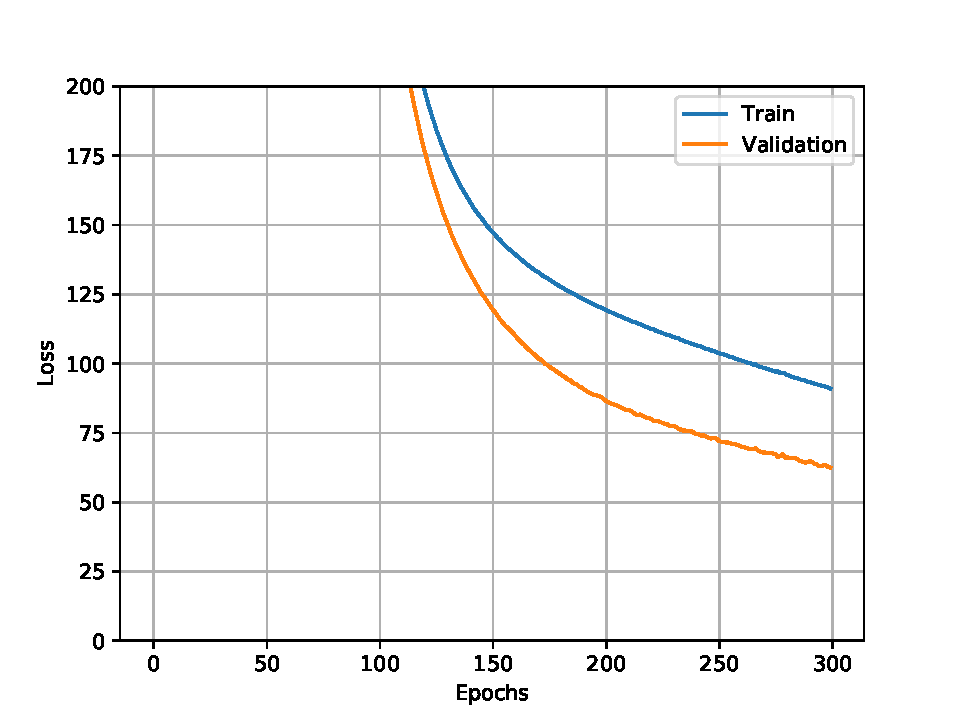
\includegraphics[width=\textwidth]{pics/figure_Boston_NN_nohidden_wd_loss.pdf}
    \caption{Loss on training and validation set during training epochs for the neural network with no hidden layers weight decay.}
    \label{fig:Boston_NN_nohidden_wd_loss}
\end{figure}

\begin{figure}
    \centering
    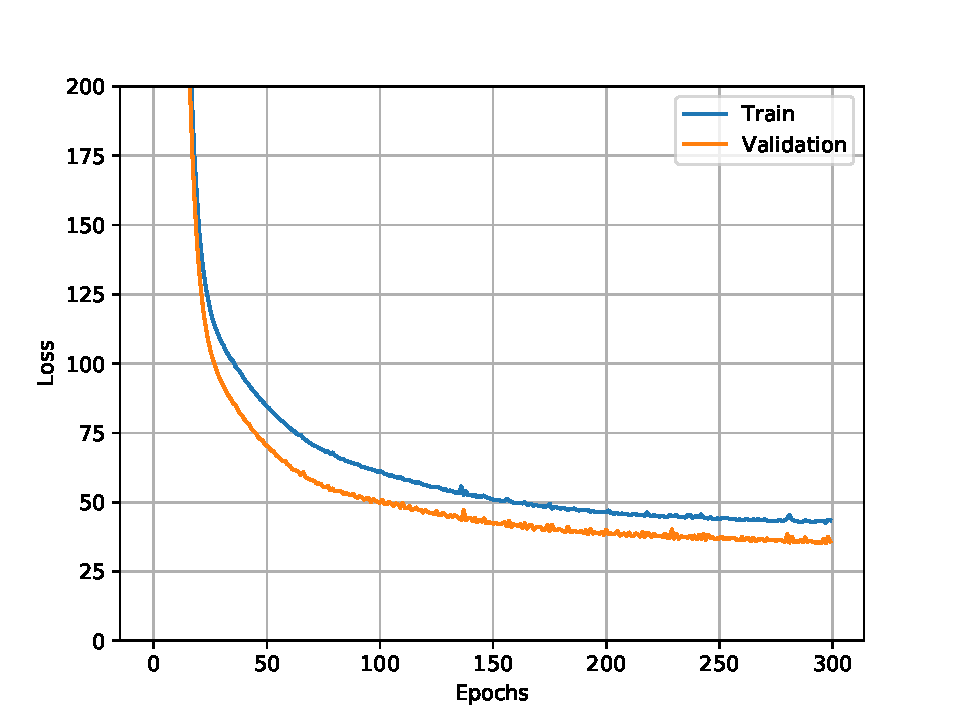
\includegraphics[width=\textwidth]{pics/figure_Boston_NN_1hidden_wd_loss.pdf}
    \caption{Loss on training and validation set during training epochs for the neural network with 1 hidden layers and weight decay. }
    \label{fig:Boston_NN_1hidden_wd_loss}
\end{figure}


\begin{figure}
    \centering
    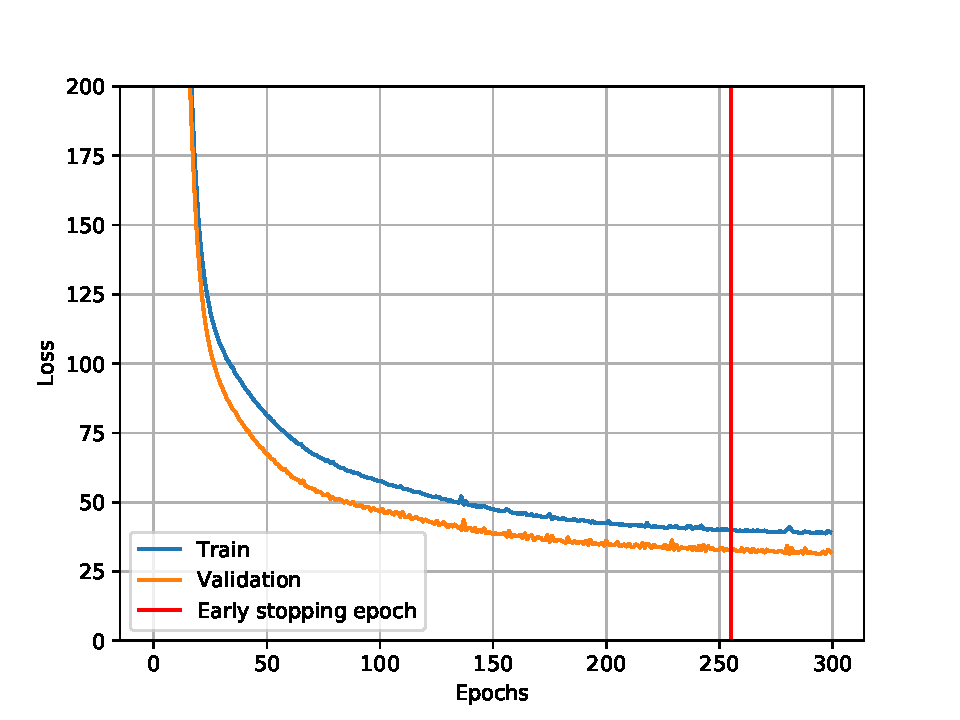
\includegraphics[width=\textwidth]{pics/figure_Boston_NN_1hidden_noreg_loss.pdf}
    \caption{Loss on training and validation set during training epochs for the neural network with one hidden layer \& no regularization. These losses are the same as for the network with 1 hidden layer and early stopping up to the stopping time on epoch 255 indicated by the red vertical line. It can be seen that validation loss is somewhat flattening and decreasing in oscillations around epoch 255, which might be what made the early stopping algorithm indicate no further improvements in validation loss, given the chosen patience of 10 epochs and $\delta_{\text{min}} = 0.1$, and stop the training.}
    \label{fig:Boston_NN_1hidden_noreg_loss}
\end{figure}
\clearpage

\subsection{Regression with Bayesian Neural
Networks}\label{subsec:regression_w_bnn}
We perform regression with the Bayesian neural networks listed in table \ref{tab:Boston_BNN_performance}. All of these networks are implemented with a Gaussian likelihood with mean equal to the network output and standard deviation $\sigma$ equal to 1. We have chosen to run three kinds of BNNs. First a BNN with no hidden layers which corresponds to Bayesian linear regression. Then a BNN with one hidden layer, where we follow the example of \cite{mackay1991} and \cite{MacKay1992} and choose a Gaussian prior on the parameter weights, which we choose more specifically to be $\mathcal{N}(0,0.1)$ . Lastly a hierarchical BNN with one hidden layer, with a $\mathcal{N}(\mu,\sigma)$ prior for the network weights. The parameter $\mu$ is chosen to follow a $\text{Cauchy}(\alpha,\beta)$ distribution and the standard deviation $\sigma$ follows a $\text{Half-Normal}(\nu)$ distribution in order to avoid negative values. The hyper-prior distributions are parametric and therefore require that we specify the hyperparameters for these.
After experimenting with different choices of parameters for the hyper-prior, we choose $\alpha=0$, $\beta=1$ and $\nu=1$. All BNN models have 10 hidden neurons for ease of comparison and in order to evaluate on the same models as in section \ref{sec:regre_w_NN} but with a Bayesian approach. \\
\\
We sample from the posterior distribution of the model parameters using the NUTS algorithm examined in section \ref{sec:nuts}.
We sample from three Markov Chains in parallel to get more independent samples, as described in section \ref{sec:MCMC}, where we for each chain draw $3000$ samples from the posterior distribution. A burn-in phase of $1000$ has been chosen for each chain. For the dual averaging algorithm we chose an
acceptance probability $\delta$ of $90\%$ , as it provided us with most acceptable results. All other inputs used for the NUTS algorithm were not chosen by us, as we used the default settings in \texttt{PyMC3}. 
Predictions are made by sampling from the posterior predictive distribution. We generate a total of $3000 \times 3$ samples from the posterior predictive distribution, and to make a single best guess in terms of minimizing MSE we make a prediction by taking the mean of the posterior predictive distribution. 
\\
\\
From table \ref{tab:Boston_BNN_performance} we see that both BNNs with one hidden layer outperform the baseline model with no hidden layers. As a BNN with no hidden layers corresponds to performing Bayesian linear regression, this indicates that using Bayesian inference in a neural network is more useful than using Bayesian inference in a simple linear regression, in this particular case. We also note that all the BNN models are outperforming the non-Bayesian neural networks in terms of MSE both on the training data, but also on the unseen test data. However, it takes about $140$ times longer to run a BNN with one hidden layer than a similar non-Bayesian neural network. So even though the BNNs get a loss-wise better result in this case, it might not be so if one has a time budget lower than the runtime found in table \ref{tab:Boston_BNN_performance}.
\\
\\
However, the computational burden that comes with BNNs also comes with the benefit of producing a distribution for the predictions. This enables us to consider more possible outcomes when making predictions and to have a better idea of the uncertainty in our predictions. The posterior predictive distribution is shown as a histogram in figure \ref{fig:post_pred_noston} for different examples in the test dataset. Such a distribution can be useful in decision making. Consider the example of a property investor, who would like to invest in a certain area. If two areas, according to our model, have the same mean median price he might wish to invest in the area that has the most narrow posterior predictive distribution i.e. lowest standard deviation, so that he is least likely to be surprised by the actual median price. 
\\
\\
We have chosen to use the mean of the posterior predictive distribution for predictions, as this is usually the best measure for central tendency when the distribution is symmetric, but from figure \ref{fig:post_pred_noston} we can see that we might want to take some caution against doing this, as the posterior predictive distribution of the chosen examples show bimodal tendencies and are not symmetric. This shows how to critically evaluate our model when we have access to the distribution of a models predictions. With non-Bayesian neural networks, we only get a single point estimate for the model parameters, and do not factor in the full range of possibilities. Despite these examples we still use the mean for prediction as it provides us with acceptable results. 

\begin{table}
\caption{Performance measurement for Bayesian neural network models on Boston housing data. The Python code used to implement these Bayesian neural networks can be seen in appendix \ref{app:Boston_BNN}.}
\label{tab:Boston_BNN_performance}
\resizebox{\textwidth}{!}{%
\begin{tabular}{|l|l|l|l|}
\hline
\multicolumn{1}{|c|}{{\cellcolor{ashgrey}{
\textbf{Model}}}}   &  \multicolumn{1}{|c|}{{\cellcolor{ashgrey}{
 \textbf{Train MSE}}}} & \multicolumn{1}{|c|}{{\cellcolor{ashgrey}{
 \textbf{Test MSE}}}}           & \multicolumn{1}{|c|}{{\cellcolor{ashgrey}{
 \textbf{Runtime (s)}}}}      \\ \hline
No hidden layers &  28.480 &   17.760    &     211.63      \\ \hline
1 hidden layer    &  11.391  & 9.340        &    1496.69                     \\ \hline
Hierarchical with 1 hidden layer     &      14.135          &  10.869  &  1851.46   \\ \hline
\end{tabular}
}
\end{table}
\begin{figure}
    \centering
    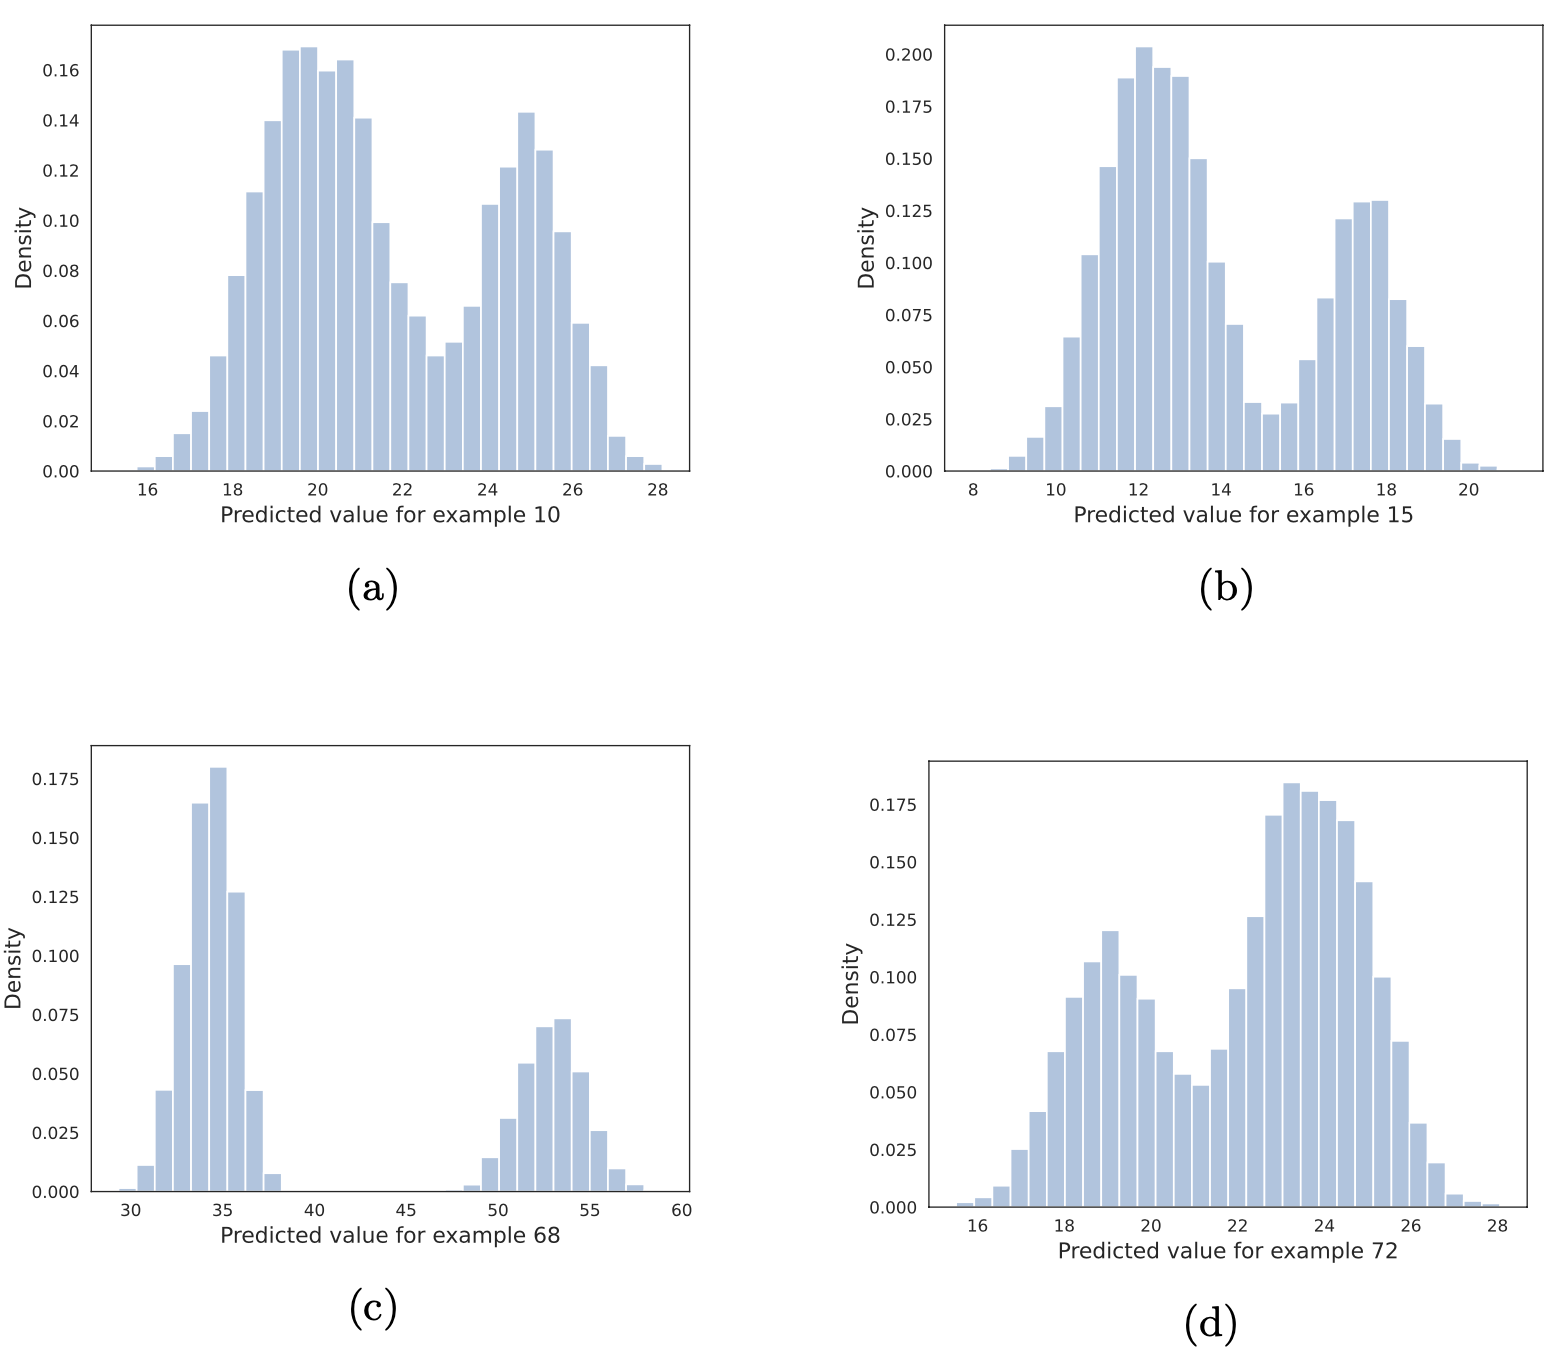
\includegraphics[width=\textwidth]{pics/post_pred_Boston.png}
    \caption{A histogram of predictions generated by samples from from the posterior predictive distribution for example 10, 15, 68 and 72 in the test dataset. The predictions are based on the 1 hidden layer BNN model}
    \label{fig:post_pred_noston}
\end{figure}

\clearpage
\section{Predicting Defaults of Credit Card Clients} \label{sec:credit_default}
The default of credit card clients dataset contains information collected by a Taiwan bank in 2005, on $30.000$ credit card clients. The data contains 25 variables, which are represented in table \ref{tab:credit_card_features}. Due to the computational complexity of the BNN model, we choose to subsample our dataset, such that it only contains $300$ train examples and $100$ test examples. We also perform the same splits of the data as in section \ref{sec:Boston_housing}, meaning that 30 \% of the data are contained in a test set, and the remaining data are afterwards split into 70 \% training data and 30 \% validation data. The data are shuffled before splitting, to prevent that it should be sorted in an undesired way.
\\
\\
The default of credit card clients dataset has earlier been used by \cite{Yeh2009TheCO} for predicting the probability of default for customers in Taiwan. The objective for our analysis is the same, to predict the probability of default on next months payment. This probability can then be used to predict defaults and expected losses. A predictive model, that can predict the default probability of the next credit card payment, could be very useful for a banks risk management unit in order to detect which customers should be allowed to own a credit card and which should be denied. 
\\
\\
The data does not contain an equal fraction of the two classes, since examples with the true label of default only constitutes $22.12\%$. Such a problem is often referred to as a class imbalance problem in binary classification and has been examined a lot through the years. \cite{imbalane_danquah2020} suggest to use methods such as oversampling and undersampling for imbalanced class problems, but this will not be performed as we simply wish to evaluate the networks performance on classification. We simply note that a model can easily get an accuracy score of around $80\%$ by just predicting the majority class for all examples without necessarily learning any patterns. 



\begin{table}\label{tab:credit_card_features}
\caption{Table of features in credit card default data. Data contains 30.000 examples each with 25 features. Data can be downloaded on:\\ \href{https://archive.ics.uci.edu/ml/datasets.php}{https://archive.ics.uci.edu/ml/datasets.php}}
\resizebox{\textwidth}{!}{%
\begin{tabular}{|l|l|}
\hline
\multicolumn{1}{|c|}{{\cellcolor{ashgrey}{
 \textbf{Feature name}}}} & \multicolumn{1}{|c|}{{\cellcolor{ashgrey}{
 \textbf{Feature description}}}}\\ \hline
LIMIT\_BAL                 &           Amount of the given credit (New Taiwan dollar): \\ & it includes both the individual consumer credit and \\ &  his/her family (supplementary) credit.           \\ \hline
SEX                        &          Gender (1 = male; 2 = female)            \\ \hline
EDUCATION                  &         Education (1 = graduate school; 2 = university; \\ &  3 = high school; 4 = others).             \\ \hline
MARRIAGE                   &         Marital status (1 = married; 2 = single; 3 = others)             \\ \hline
AGE                        &            Age (year)           \\ \hline
PAY\_0                     &         Repayment status in September, 2005 \\ &  -2=no consumption, -1=pay duly \\ &  0=the use of revolving credit, 1=payment delay for one month \\ &  2=payment delay for two months, 3=payment delay for three months\\ & $\vdots$ \\ &  8=payment delay for eight months, 9=payment delay for nine months and above         \\ \hline
PAY\_2                     &        
Repayment status in August, 2005 (scale same as above)\\ \hline
PAY\_3                     &          Repayment status in July, 2005 (scale same as above)            \\ \hline
PAY\_4                     &            Repayment status in June, 2005 (scale same as above)          \\ \hline
PAY\_5                     &            Repayment status in May, 2005 (scale same as above)          \\ \hline
PAY\_6                     &           Repayment status in April, 2005 (scale same as above)           \\ \hline
BILL\_AMT1                 &           Amount of bill statement in September, 2005 (NT dollar)           \\ \hline
BILL\_AMT2                 &            Amount of bill statement in August, 2005 (NT dollar)          \\ \hline
BILL\_AMT3                 &              Amount of bill statement in July, 2005 (NT dollar)        \\ \hline
BILL\_AMT4                 &            Amount of bill statement in June, 2005 (NT dollar)          \\ \hline
BILL\_AMT5                 &           Amount of bill statement in May, 2005 (NT dollar)           \\ \hline
BILL\_AMT6                 &           Amount of bill statement in April, 2005 (NT dollar)           \\ \hline
PAY\_AMT1                  &               Amount of previous payment in September, 2005 (NT dollar)       \\ \hline
PAY\_AMT2                  &          Amount of previous payment in August, 2005 (NT dollar)            \\ \hline
PAY\_AMT3                  &              Amount of previous payment in July, 2005 (NT dollar)        \\ \hline
PAY\_AMT4                  &              Amount of previous payment in June, 2005 (NT dollar)        \\ \hline
PAY\_AMT5                  &              Amount of previous payment in May, 2005 (NT dollar)        \\ \hline
PAY\_AMT6                  &           Amount of previous payment in April, 2005 (NT dollar)           \\ \hline
default payment next month &             Default payment (1=yes, 0=no)         \\ \hline
\end{tabular}}
\end{table}


\clearpage
\subsection{Classification with Neural Networks}\label{sec:clas_w_nn}
We perform predictions on default probabilities of credit card clients using the networks in table \ref{tab:credit_NN_performance}. All of these networks use the $\tanh$ activation function from equation \ref{eq:tanh} in every hidden layer and a sigmoid activation from equation \ref{eq:sigmoid} for the output layer. All networks have 10 neurons in each hidden layer and are trained with 1000 epochs using ADAM from section \ref{sec:ADAM}. These settings were selected after experimenting with different other options and the settings are the same for all the neural networks so that we can compare them on their individual differences. The training and validation loss for each training epoch of the networks can be seen in figure \ref{fig:Credit_NN_nohidden_wd_loss}, figure \ref{fig:Credit_NN_1hidden_wd_loss} and figure \ref{fig:Credit_NN_1hidden_noreg_loss}.\\




\begin{table} 
\caption{Performance measurement for neural network models on Boston Housing data. Early stopping ran 194 epochs. The Python code used to implement these neural networks can be seen in appendix \ref{app:Credit_NN}.}
\label{tab:credit_NN_performance}
\resizebox{\textwidth}{!}{%
    \begin{tabular}{|l|l|l|l|}
    \hline
    \multicolumn{1}{|c|}{{\cellcolor{ashgrey}{
     \textbf{Model}}}} & \multicolumn{1}{|c|}{{\cellcolor{ashgrey}{
     \textbf{Train cross-entropy loss}}}}       & \multicolumn{1}{|c|}{{\cellcolor{ashgrey}{
     \textbf{Test cross-entropy loss}}}} & \multicolumn{1}{|c|}{{\cellcolor{ashgrey}{
     \textbf{Runtime (s)}}}} \\ \hline
    No hidden layers \& weight decay &  47.841  &   67.646  &     38.08    \\ \hline
    1 hidden layer \& no regularization &   0.498  &   0.565  &   38.80        \\ \hline
    1 hidden layers \& weight decay &  0.513  &  0.558   &     28.44     \\ \hline
    1 hidden layers \& early stopping  &  0.503   &   0.564   &      6.15    \\ \hline
    \end{tabular}
}
\end{table}
\noindent
We examine a network with no hidden layers and weight decay as this correspond to logistic regression with weight decay to see if a complex model like neural networks are beneficial for this task instead of using simple logistic regression. We see from table \ref{tab:Boston_NN_performance} that no hidden layers i.e. logistic regression has a much larger train and test loss indicating that neural networks are indeed more useful for this task. 
\\
\\
The neural network with one hidden layer and no regularization gets a smaller train loss but larger test loss than the other one hidden layer networks. This indicates that this network is overfitting, which is also apparent in figure \ref{fig:Credit_NN_1hidden_noreg_loss}. The NN with one hidden layer and weight decay is regularized and provides a larger training loss but smaller test loss indicating that weight decay has mitigated the overfitting. The NN with one hidden layer and early stopping has a slightly larger test loss than the NN with one hidden layer and weight decay, but it shows a small improvement in test loss compared to the network with no regularization and a substantially shorter runtime. This is caused by sudden continually increase in the validation error as shown in figure \ref{fig:Credit_NN_1hidden_noreg_loss}. We see here that early stopping stops training at the exact time, that the validation error starts increasing, and this happens as we chose patience and $\delta_{\text{min}}$ to both be zero. These values were chosen by seeing that the validation error was smoothly increasing when training the network with no regularization. 

\begin{figure}[h!]
    \centering
    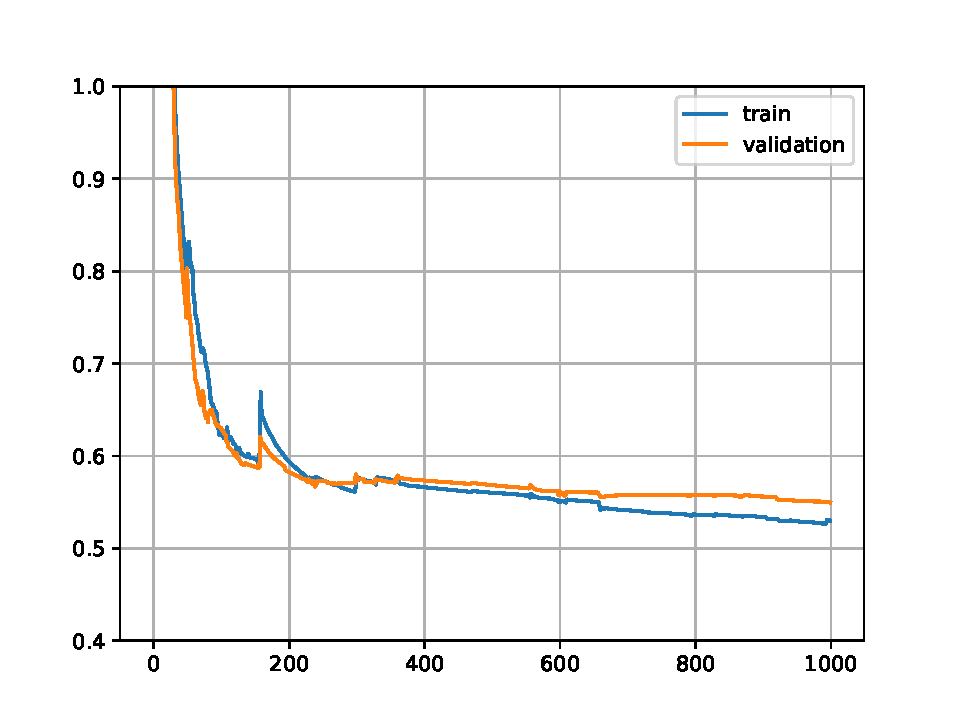
\includegraphics{pics/figure_Credit_NN_1hidden_wd_loss.pdf}
    \caption{Loss on training and validation set during training epochs for the neural network with no hidden layers \& weight decay.}
    \label{fig:Credit_NN_nohidden_wd_loss}
\end{figure}

\begin{figure}
    \centering
    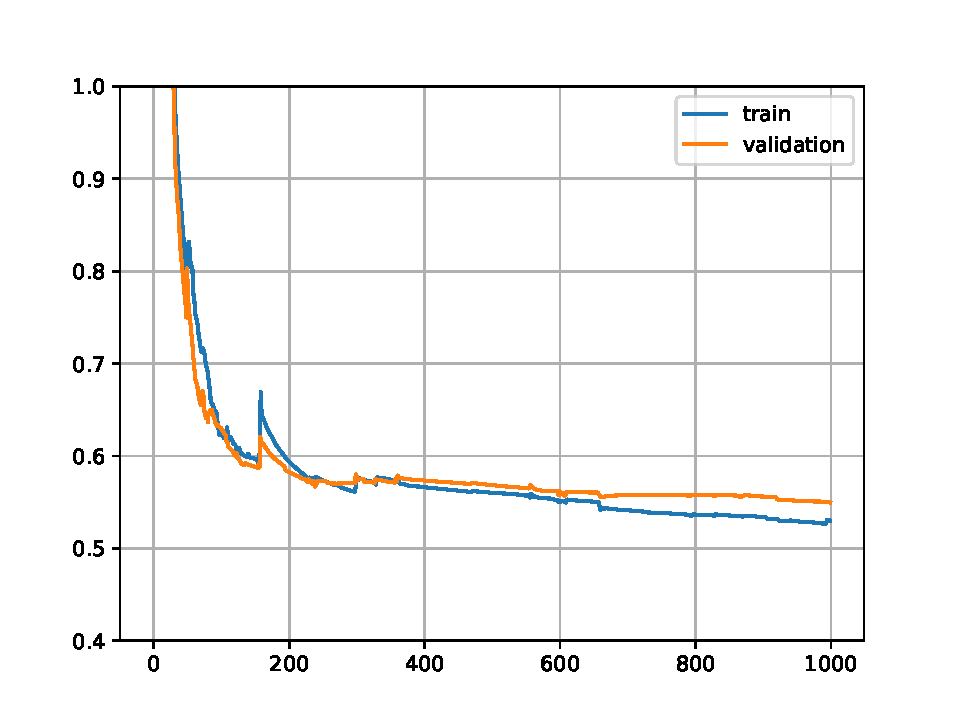
\includegraphics{pics/figure_Credit_NN_1hidden_wd_loss.pdf}
    \caption{Loss on training and validation set during training epochs for the neural network with 1 hidden layers \& weight decay. }
    \label{fig:Credit_NN_1hidden_wd_loss}
\end{figure}


\begin{figure}
    \centering
    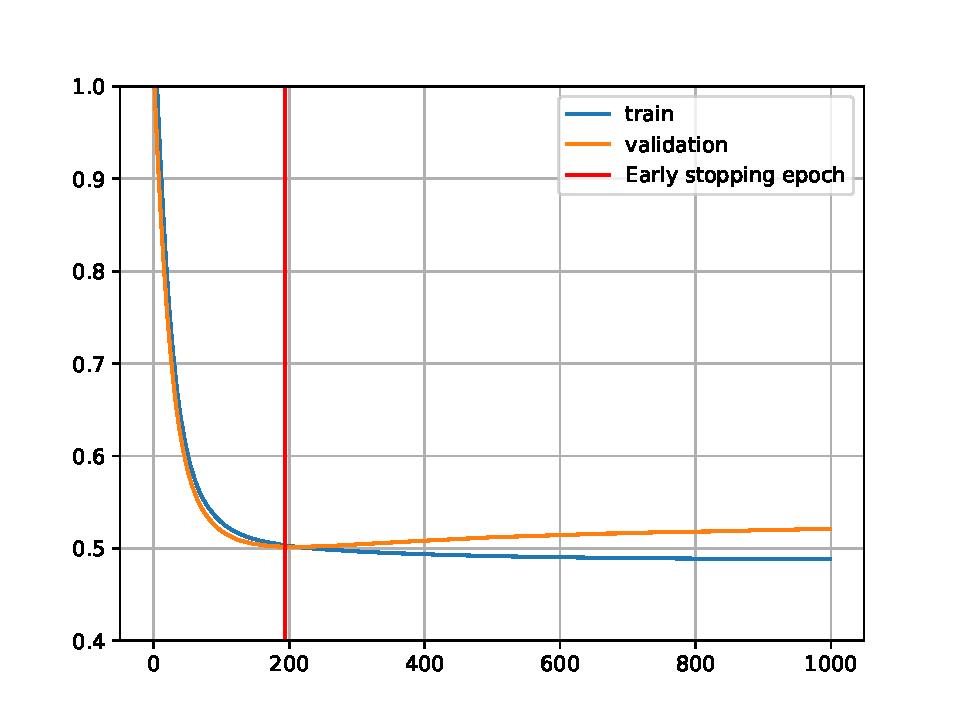
\includegraphics{pics/figure_Credit_NN_1hidden_noreg_loss.pdf}
    \caption{Loss on training and validation set during training epochs for the neural network with 1 hidden layers \& no regularization. These losses are the same as for the network with 1 hidden layer and early stopping up to the stopping time on epoch 194, indicated by the red vertical line. It can be seen that validation loss is smoothly increasing, which is what made the early stopping algorithm indicate no further improvements in validation loss and stop the training, given the chosen patience of 0 epochs and $\delta_{\text{min}} = 0$.}
    \label{fig:Credit_NN_1hidden_noreg_loss}
\end{figure}
\clearpage
\subsection{Classification with Bayesian Neural Networks}
In this section we predict default probabilities with the Bayesian neural networks listed in table \ref{tab:credit_BNN_performance}. All these models are implemented with tanh activation function as in the previous section with non-Bayesian neural network. All three models are implemented with a $\operatorname{Bernoulli}\lr{p}$ likelihood, where the bias $p$ is equal to the outputted probability of the network. The BNN with no hidden layers is used for comparing performance of the models to a simple Bayesian logistic regression. The BNN with one hidden layer has a $\mathcal{N}\lr{0,1}$ prior distribution placed on the network parameters. The hierarchical BNN with one hidden layer, has a $\mathcal{N}\lr{\mu,\sigma}$ prior for the network weights, where $\mu$ and $\sigma$ are distributed by a Cauchy and half-normal distribution respectively, as in the regression evaluation. \\
\\
Sampling from the posterior distribution is performed using NUTS with three Markov chains, that runs in parallel, to avoid dependence between samples. For each chain we choose to draw 1500 samples, as running more than 1500 samples per chain resulted in the system exceeded its memory limit. Like before, we use a burn-in phase of 1000 samples for each chain, since we believe the Markov chains must have converged to the posterior by then. For the NUTS-algorithm we choose an
acceptance probability $\delta$ of $90\%$ and for all other inputs we use the default setting of \texttt{PyMC3}. Predictions are performed by sampling $1500 \times 3$ from the posterior predictive distribution and then take the mean across samples to make a single best guess for the default probability. \\
\\
In table \ref{tab:credit_BNN_performance} we see that both the BNN with one hidden layer and the BNN as a hierarchical model are performing better than the BNN with no hidden layers. This indicates that it is useful to use a neural network for predicting credit default probabilities compared to using Bayesian logistic regression. We see that the runtimes of the BNNs are much higher than the non-Bayesian models, and since we get the same results in terms of cross-entropy loss, it is not beneficial to use BNNs instead of NNs if one is only interested in getting the lowest loss pr. runtime.  \\

\begin{table} 
\caption{Performance measurement for Bayesian neural network models on credit card default data. The Python code used to implement these Bayesian neural networks can be seen in appendix \ref{app:Credit_BNN}.}
\label{tab:credit_BNN_performance}
\resizebox{\textwidth}{!}{%
    \begin{tabular}{|l|l|l|l|}
    \hline
    \multicolumn{1}{|c|}{{\cellcolor{ashgrey}{
     \textbf{Model}}}} & \multicolumn{1}{|c|}{{\cellcolor{ashgrey}{
     \textbf{Train cross-entropy loss}}}}       & \multicolumn{1}{|c|}{{\cellcolor{ashgrey}{
     \textbf{Test cross-entropy loss}}}} & \multicolumn{1}{|c|}{{\cellcolor{ashgrey}{
     \textbf{Runtime (s)}}}} \\ \hline
    No hidden layers  &  0.774  &  0.685   &    20.332      \\ \hline
    1 hidden layer &  0.523   &  0.539   &   1233.58       \\ \hline
    Hierarchical with 1 hidden layer  &  0.523  &   0.539  &   3640.28       \\ \hline
    \end{tabular}
}
\end{table}
\noindent
The benefits of the BNNs are instead found in the produced distribution of the predictive posterior.From a risk management perspective, this could be interesting to get an idea of the uncertainty of the models prediction of default probability. The mean probability of defaulting might be $45 \%$ for two different clients, but the uncertainty in this quantity might be significantly different. This uncertainty can be examined by taking a look at the posterior predictive distribution. In figure \ref{fig:ppc_credit} we have illustrated the posterior predictive distribution generated by the one hidden layer BNN for example 5, 11, 25 and 88 in the test dataset. We see that sometimes the model is quite confident about its predictions as in subfigure (c) and (d), but for other examples the uncertainty, expressed by the standard deviation of the distribution, is quite high like in subfigure (a) and (b). A bank could use this to decide not to give credit to a client if the uncertainty of the default probability is too high, like the client corresponding to subfigure (a) of figure \ref{fig:ppc_credit}.
\\
\\
In practice one might use the predicted default probabilities, that we use for our evaluation, to predict if the client will default or not. One can do this by classifying the most probable class, which means predicting default if the probability is more than $50 \%$.
This might however not be the most reasonable approach, if one prefers to wrongly classify one class more than the other. We might for example imagine that providing credit to a client that defaults next month would be much worse than denying a client that does not default next month. In this case it can make sense to choose another classification boundary than $50\%$. 
\\
\\
This classification boundary can be determined by the loss of wrongly predicting certain classes and can be set so that the expected loss do not exceed a certain value. Choosing a proper classification boundary for this case will however not be pursued further, as we performed our evaluation using the default probabilities instead of the labels, which would depend on the choice of such classification boundary.
  

\begin{figure}
    \centering
    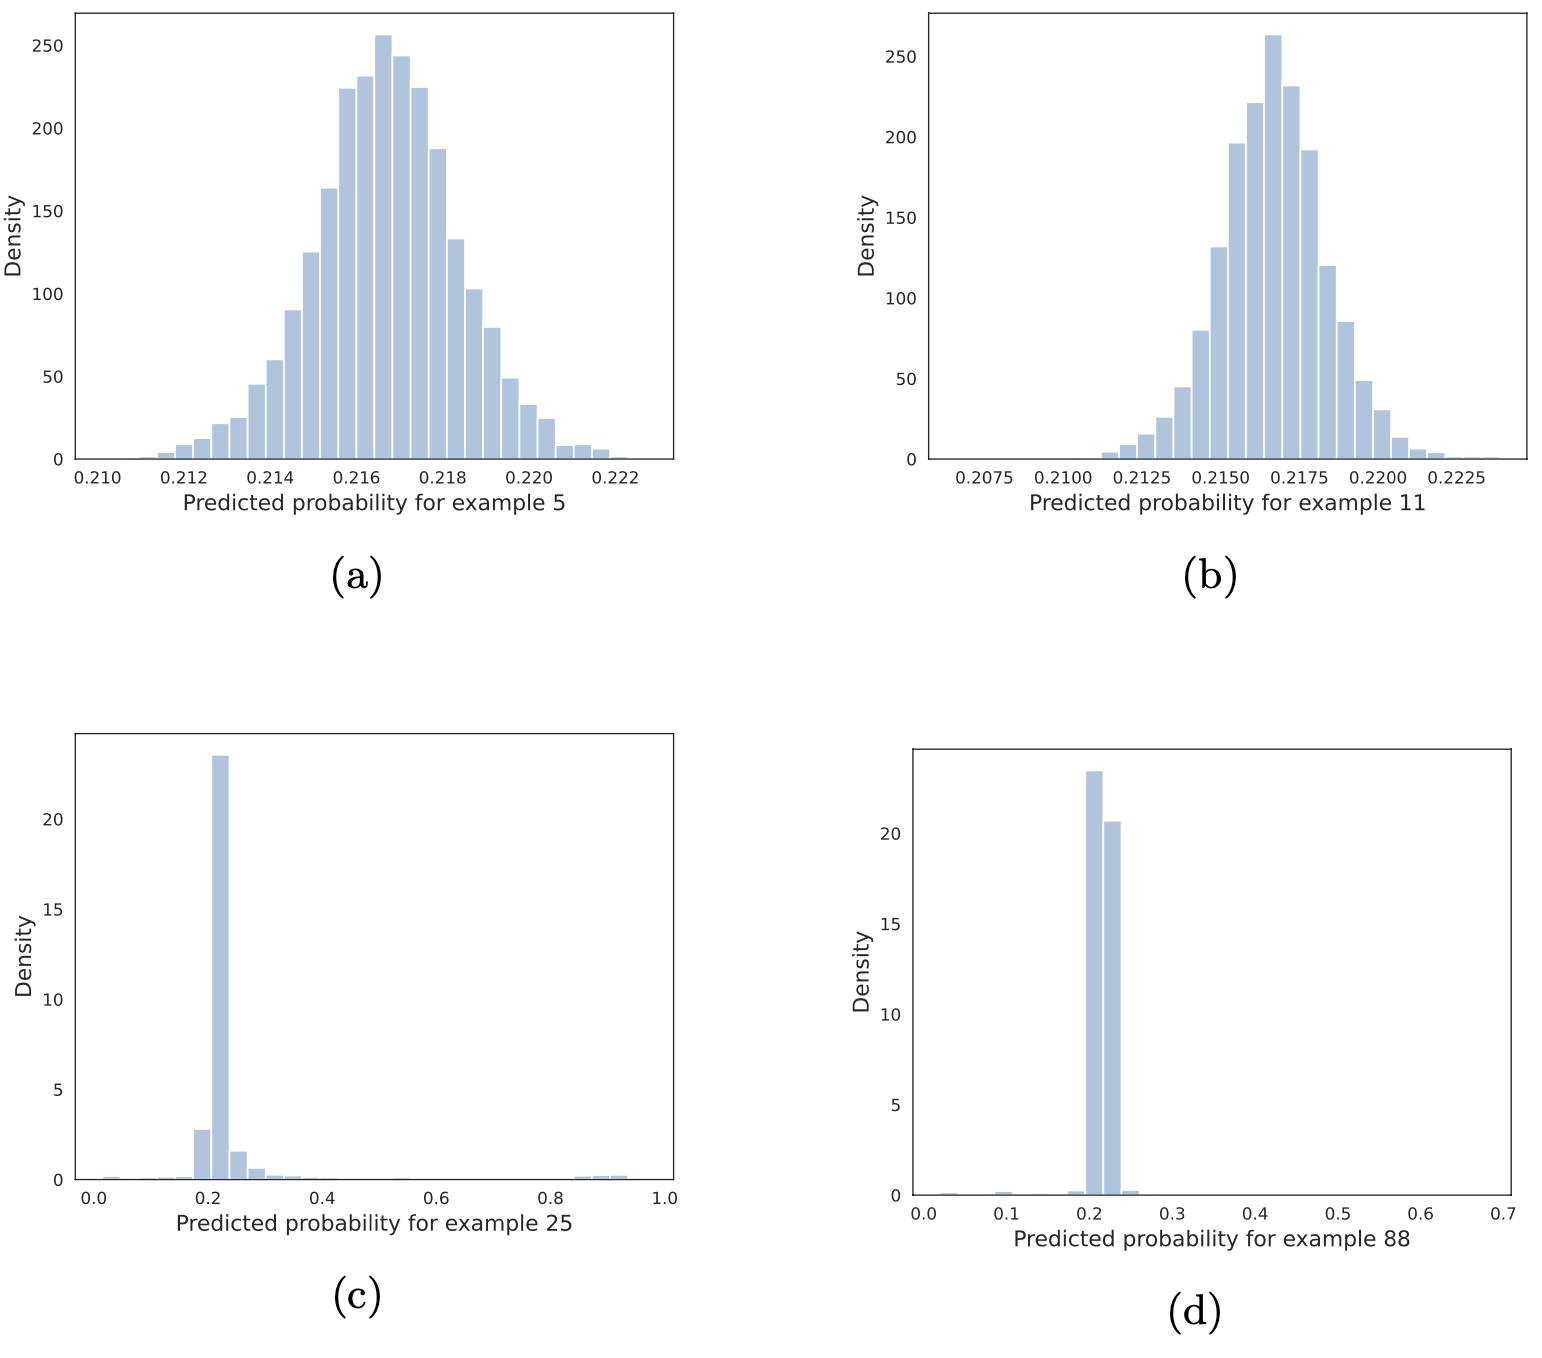
\includegraphics[width=\textwidth]{pics/post_pred_credit.png}
    \caption{A histogram of predictions generated by sampling from the posterior predictive distribution for example 5, 11, 25 and 88 in the test dataset. The predictions are based on the 1 hidden layer BNN model.}
    \label{fig:ppc_credit}
\end{figure}


